\section{The clone databases}
\label{ch:impementation-clones}

\begin{wrapfigure}{r}{0.5\textwidth}
  \vspace{-20pt}
  \begin{center}
    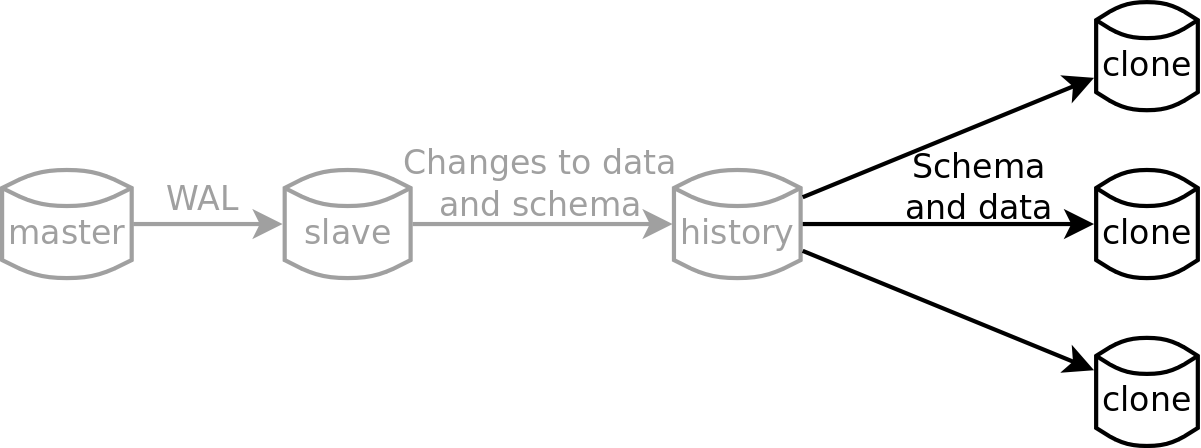
\includegraphics[width=0.48\textwidth]{img/architecture-clones}
  \end{center}
  \vspace{-20pt}
  \caption{The clone part of the architecture}
  \vspace{-10pt}
\end{wrapfigure}

A clone database is a replica of the master database.
The user can query the clone just like she would query the master.
It is a standard Postgres database that uses the \textit{PL/pgSQL} and \textit{dblink} extensions.
The user creates a new, empty database and runs the script \textit{clone.py} to initialize it as a clone.
The script reads the schema information from the history database and initializes the clone accordingly.

Like the history database the clone database must have the same minor version as the master.
If the master has the version 9.3.3 that means that the clone databases must have a version number that starts with 9.3.

The initialization script creates schemas in the clone database to match those in the master database.
The tables in the clone are lazy loading.
This means that a table is empty until a user queries it for the first time.
The clone then fetches its content from the history database.
This is implemented with a view which the user queries and an accompanying data table which stores the data once it has been fetched from the history.

The data tables live in a schema called \textit{marty}.
They have the same name as the data tables in the history database (see chapter \ref{ch:implementation-history-data}).
The columns are identical to the columns in the original table in the master database, there are no extra columns and their names are identical to the column names in the original table.
See figure \ref{fig:clone-tables-2} for an example of a data table.

\begin{figure}[h!]
  \centering
    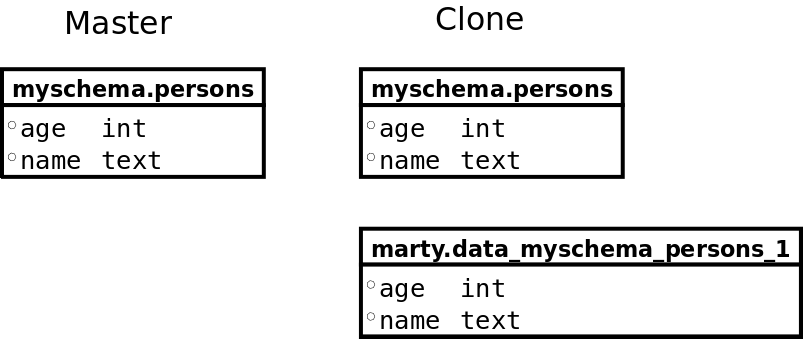
\includegraphics[width=0.6\textwidth]{clone-tables}
  \caption{Table layout in a clone database}
  \medskip
  \small
  The table \textit{persons} is actually a view that returns results from the table \textit{data\_myschema\_persons\_1} which is in the \textit{marty} schema.
  \label{fig:clone-tables-2}
\end{figure}

When the user queries a table in the clone database like she would query it in the master she is actually querying the view that Marty creates.
It executes a PL/pgSQL function, \textit{view\_select}, which returns the contents of the original table in the master.
The function is created by Marty when the clone is initialized.
It receives one argument, the name of the view that is being queried, and fetches the data for it from the corresponding data table.
When the view is queried for the first time the view\_select function fetches the data from the history database and inserts it into the data table before returning the results.
See listing \ref{lst:view-select} for the source code of the view\_select function.

\lstset{
  language=SQL,
  morekeywords={
    FUNCTION, RETURNS, SETOF, RECORD, DECLARE, BEGIN,
    IF, RAISE, NOTICE, RETURN, QUERY, LANGUAGE,
    int, text
  }
}
\begin{lstlisting}[caption={The view\_select function},label={lst:view-select},numbers=left,xleftmargin=2em]
CREATE FUNCTION view_select(my_view_name text) RETURNS SETOF RECORD AS $$
DECLARE
  view_info RECORD;
BEGIN
  SELECT * FROM marty.bookkeeping WHERE view_name = my_view_name INTO view_info;
  IF NOT view_info.cached THEN
    RAISE NOTICE 'fetching %', view_info.view_name;
    EXECUTE ' INSERT INTO ' || view_info.local_table ||
      ' SELECT ' || view_info.coldef ||
      ' FROM dblink(''' || coninfo() || ''', ''' || view_info.remote_select_stmt || ''')'
      ' AS ' || view_info.temp_table_def;
	UPDATE marty.bookkeeping SET cached = true WHERE view_name = my_view_name;
  END IF;
  RETURN QUERY EXECUTE 'SELECT ' || view_info.coldef || ' FROM ' || view_info.local_table;
END;
$$ LANGUAGE plpgsql;
\end{lstlisting}

Marty keeps track of which data tables have been populated in the table \textit{bookkeeping}.
It is created alongside the data tables in the marty schema when the clone database is initialized and is used to store information about the data tables and views.
It stores which data table keeps the data for which view and whether it has been initialized, as well as information about how to query the history database to fetch the data for each view.
See table \ref{tbl:bookkeeping} for a list of columns in the bookkeeping table.

\begin{table}[h]
  \centering
  \textbf{bookkeeping}
  \begin{tabularx}{\textwidth}{llX}
    \textit{Column} & \textit{Type} & \textit{Description} \\
    \midrule
    view\_name & name & The name of the view \\
    local\_table & name & The name of the data table that contains the data for the view \\
    cached & boolean & True if the data table has been populated with data from the history database \\
    coldef & text & A list of columns in the data table, used by the \textit{view\_select} function when querying the data table \\
    remote\_select\_stmt & text & The select statement for the data table in the history database \\
    temp\_table\_def & text & Table definition for a temporary table, used by view\_select \\
  \end{tabularx}
  \caption{The columns of the bookkeeping table}
  \label{tbl:bookkeeping}
\end{table}

The \textit{cached} column is a boolean which tells the view\_select function whether the data table has been populated with data from the history database (line 6 in listing \ref{lst:view-select}).
It defaults to false as all data tables start empty.
The function uses the \textit{coldef} value when it queries the data table.
It is a comma separated list of the columns in the data table and is used to construct the select query (line 14).
When the view\_select function queries the history database it uses the \textit{remote\_select\_stmt} as the query (lines 7 to 11).
It is a select query that returns all rows from the data table in the history.
The \textit{dblink} function from the dblink extension is used to query the history database (line 10).
It receives two parameters; a connection string and the query to run.

The connection string is generated when the clone database is initialized.
Marty creates a function, \textit{coninfo}, that returns this string.
This makes it trivial to update the connection string later in a running clone database if the setup of the history database changes, as only this one-line function needs to be redefined instead of the whole view\_select function.
The query that returns the data from the history database is created when Marty initializes the clone and is saved in the \textit{remote\_select\_stmt} column in the bookeeping table.


\begin{lstlisting}[caption={An example of a SELECT query with a table alias},label={lst:table-alias-query}]
SELECT * FROM dblink('dbname=mydb', 'SELECT age, name FROM persons') AS p(age int, name text)
\end{lstlisting}

The dblink query must have an alias part where the names and types of the columns in the result rows are specified.
This is because the dblink function is declared to return a set of \textit{records}.
Postgres does not know the format of the records so the user must provide this information with the alias\footnote{http://www.postgresql.org/docs/9.3/static/contrib-dblink-function.html}.
See listing \ref{lst:table-alias-query} for an example.
The part after \textit{AS} tells Postgres what to expect in the query results.
This part is unique to each data table in the clone database.
It is saved in the \textit{temp\_table\_def} column in the bookkeeping table and is appended to the dblink query in the view\_select function (line 11).